\documentclass[8pt]{article}
\usepackage[UTF8]{ctex}
\usepackage[a4paper]{geometry}
%\setCJKmainfont[ItalicFont=Noto Serif CJK SC Bold, BoldFont=Noto Serif CJK SC Black]{Noto Serif CJK SC}

\usepackage{amsthm,amsmath,amssymb}
\usepackage{graphicx}
\usepackage{subfigure}
\usepackage{amsmath}
\usepackage{tabularx}
\usepackage{color}
\usepackage{hyperref}
\usepackage{ulem}
\usepackage{multirow}
\usepackage[cache=false]{minted}
\hypersetup{
	colorlinks=true,
	linkcolor=blue
}

\usepackage{appendix}
\geometry{a4paper,centering,scale=0.8}
\geometry{left=2.0cm, right=2.0cm, top=2.5cm, bottom=2.5cm}
\usepackage[format=hang,font=small,textfont=it]{caption}
\usepackage[nottoc]{tocbibind}

\usepackage{algorithm}
\usepackage{algorithmicx}
\usepackage{algpseudocode}
\usepackage{amssymb}
\usepackage{extarrows}
\usepackage{qcircuit}
\usepackage{fancyhdr}
\usepackage{cleveref}
\usepackage{totpages}



\usepackage{pgf}
\usepackage{tikz}
\usetikzlibrary{arrows,automata}
\usetikzlibrary{arrows.meta}%画箭头用的包

\makeatletter
\def\@maketitle{%
	\newpage
	\begin{center}%
		\let \footnote \thanks
		{\LARGE \@title \par}%
		\vskip 1.5em%
		{\large
			\lineskip .5em%
			\begin{tabular}[t]{c}%
				\@author
			\end{tabular}\par}%
		\vskip 1em%
		{\large \@date}%
	\end{center}%
	\par
	\vskip 1.5em}
\makeatother

\newtheoremstyle{compact}%
{3pt}{3pt}%
{}{}%
{\bfseries}{\textcolor{red}{.}}%  % Note that final punctuation is omitted.
{.5em}{\mbox{\textcolor{red}{\thmname{#1}\thmnumber{ #2}}\thmnote{ (\textcolor{blue}{#3})}}}
\theoremstyle{compact}
\newtheorem{innercustomgeneric}{\customgenericname}
\providecommand{\customgenericname}{}
\newcommand{\newcustomtheorem}[2]{%
	\newenvironment{#1}[1]
	{%
		\renewcommand\customgenericname{#2}%
		\renewcommand\theinnercustomgeneric{##1}%
		\innercustomgeneric
	}
	{\endinnercustomgeneric}
}

\DeclareMathOperator{\card}{card}

\newtheorem{theorem}{定理}
\newtheorem{lemma}{引理}
\newtheorem{definition}{定义}
\newtheorem{proposition}{命题}
\newtheorem{corollary}{推论}
\newtheorem{remark}{注}
\newtheorem{Proof}{证明}

\def\obj#1{\textbf{\uline{#1}}}
\def\num#1{\textnormal{\textbf{\mbox{\textcolor{blue}{(#1)}}}}}
\def\le{\leqslant}
\def\ge{\geqslant}
\def\im{\text{im }}
\def\Pr#1{\text{Pr}\left[{#1}\right]}
\def\E#1{\mathbb{E}\left[{#1}\right]}
\def\Var#1{\text{Var}\left[{#1}\right]}


\title{\heiti\zihao{1} 计算理论导论 \ 第一次作业}
\author{\kaishu\zihao{-3} 周书予\\2000013060@stu.pku.edu.cn}

\CTEXoptions[today=old]
\date{\today}

\begin{document}
\fancypagestyle{plain}{
	\fancyhf{}
	\lhead{计算理论导论}
	\chead{2022 Spring}
	\rhead{Introduction to Theory of Computation}
	\cfoot{第 \thepage 页, 共 \pageref{TotPages} 页}
}
\pagestyle{plain}



\crefname{theorem}{定理}{定理}
\crefname{lemma}{引理}{引理}
\crefname{figure}{图}{图}
\crefname{table}{表}{表}	
\maketitle

\section{}
\subsection{}
\begin{center}
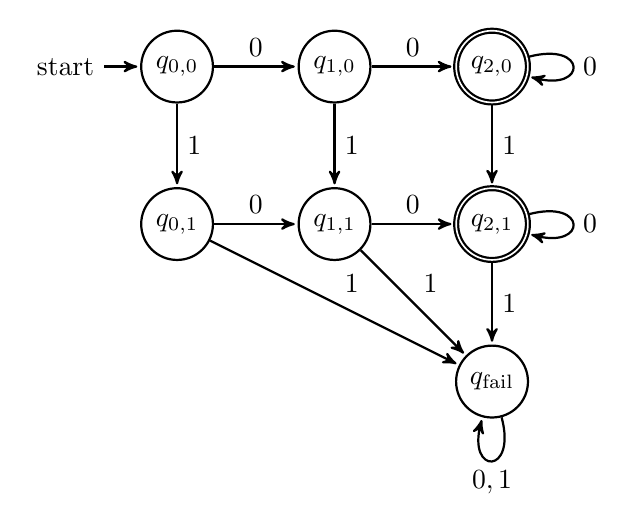
\begin{tikzpicture}[->,>=stealth',shorten >=1pt,auto,node distance=2cm,
    thick,base node/.style={circle,draw,minimum size=16pt}, real node/.style={double,circle,draw,minimum size=35pt}]

	\node[initial, state] (1) {$q_{0, 0}$};
	\node[state] (2) [right of=1] {$q_{1, 0}$};
	\node[state, accepting] (3) [right of=2] {$q_{2, 0}$};
	\node[state] (4) [below of=1] {$q_{0, 1}$};
	\node[state] (5) [below of=2] {$q_{1, 1}$};
	\node[state, accepting] (6) [below of=3] {$q_{2, 1}$};
	\node[state] (7) [below of=6] {$q_{\text{fail}}$};
	
	\path[]
	(1) edge node {$0$} (2)
	(2) edge node {$0$} (3)
	(4) edge node {$0$} (5)
	(5) edge node {$0$} (6)

	(1) edge node {$1$} (4)
	(2) edge node {$1$} (5)
	(3) edge node {$1$} (6)
	(4) edge node {$1$} (7)
	(5) edge node {$1$} (7)
	(6) edge node {$1$} (7)
	(3) edge [loop right] node {$0$} (3)
	(6) edge [loop right] node {$0$} (6)
	(7) edge [loop below] node {$0, 1$} (7);
		
\end{tikzpicture}
\end{center}
\subsection{}
\begin{center}
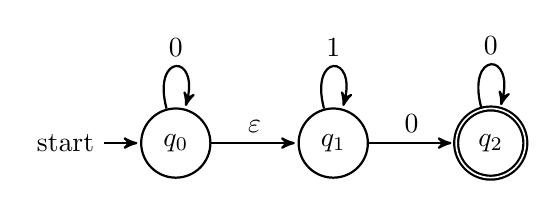
\begin{tikzpicture}[->,>=stealth',shorten >=1pt,auto,node distance=2cm,
    thick,base node/.style={circle,draw,minimum size=16pt}, real node/.style={double,circle,draw,minimum size=35pt}]

	\node[initial, state] (1) {$q_{0}$};
	\node[state] (2) [right of=1] {$q_1$};
	\node[state, accepting] (3) [right of=2] {$q_2$};
	
	\path[]
	(1) edge node {$\varepsilon$} (2)
	(2) edge node {$0$} (3)
	(1) edge [loop above] node {$0$} (1)
	(2) edge [loop above] node {$1$} (2)
	(3) edge [loop above] node {$0$} (3);
		
\end{tikzpicture}
\end{center}

\section{}
\subsection*{分析}
	需要让可接受的串在到达终止状态后, 无论再加上什么后缀都无法再到达一个终止状态. 因此只需要从识别 $A$ 的 DFA 的终止状态集合中剔除掉一些不合法的即可.
\subsection*{证明}
	假设 DFA $M = (Q, \Sigma, \delta, q_0, F)$ 识别语言 $A$, 考虑修改其终止状态集合得到新的 DFA $M' = (Q, \Sigma, \delta, q_0, F')$, 其中
	$$F' = \{q \in F | \nexists q' \in F \text{ s.t. }q'\text{ is reachable from }q\}$$

	称 $q'$ 可以被 $q$ 到达, 如果存在串 $w \in \Sigma^*$(记$|w| = l$), 状态序列$r_0, r_1, \cdots, r_l$ 满足 $r_0 = q_0, r_{i} = \delta(r_{i-1}, w_i)\ (\forall 1 \le i \le l)$, 以及两个非负整数 $0 \le m < n \le l$ 满足 $r_{m} = q, r_{n} = q'$.

	不难验证 $M'$ 可以识别 \textsf{NOEXTEND}$(A)$, 因此正则语言在 \textsf{NOEXTEND} 下是封闭的. \hfill $\square$ 

\section{}
\subsection*{分析}
	需要构造新的自动机来“交替”匹配 $a, b$ 两串. 由于匹配顺序是不确定的, 需要引入 nondeterminism.
\subsection*{证明}
	假设 DFA $M_1 = (Q_1, \Sigma, \delta_1, q_1, F_1), M_2 = (Q_2, \Sigma, \delta_2, q_2, F_2)$ 分别识别语言 $A, B$, 考虑构造 NFA $M_3 = (Q_3, \Sigma, \delta_3, q_3, F_3)$, 其中
	\begin{itemize}
		\item $Q_3 = Q_1 \times Q_2$.
		\item $\delta_3((q_x, q_y), a) = \{(\delta_1(q_x, a), q_y), (q_x, \delta_2(q_y, a))\}$.
		\item $q_3 = (q_1, q_2)$.
		\item $F_3 = F_1 \times F_2$.
	\end{itemize}

	不难验证 $M_3$ 可以识别语言 $A\ \textbf{shuffle}\ B$, 因此正则语言在 \textbf{shuffle} 下是封闭的. \hfill $\square$ 

\section{}
	考虑 $C = \{1^{kn} | n \ge 0\}$, 显然 $C$ 可以由 $k$ 个状态的 DFA 识别. 

	对于任意有 $k-1$ 个状态 $q_1, \cdots, q_{k-1}$ 的 DFA , 考虑在输入了串 $1, 11, \cdots, 1^{k}$ 后, 根据鸽巢原理, 至少存在其中两个串使得该 DFA 在输入了这两个串后到达了相同的状态, 不妨假设分别是 $1^m$ 和 $1^n$ $(1 \le m < n \le k)$, 这说明该 DFA 在输入 $1^k$ 和 $1^{n-m+k}$ 后也会到达相同的状态, 但显然 $1^k \in C$ 而 $1^{n-m+k} \notin C$, 所以产生了矛盾.
\section{}
\subsection*{(a))}
	假设 $A = \{0^n1^m0^n | m, n \ge 0\}$ 是正则语言, 则根据 pumping lemma 存在 pumping length $p$. 考虑 $s = 0^p1^p0^p \in A$, 将其划分成 $s = xyz$, 由于$|xy| \le p$, $y$只能包含 $0$ 字符, 而 $|y| > 0$ 导致了 $xyyz \notin A$, 产生矛盾. 故 $A = \{0^n1^m0^n | m, n \ge 0\}$ 不是正则语言.
\subsection*{(b)}
	由于正则语言在取补集下是封闭的, $B = \{w \in \{0, 1\}^*| w \text{ is not a palindrome}\}$ 是正则语言当且仅当 $\overline{B} = \{w \in \{0, 1\}^*| w \text{ is a palindrome}\}$ 是正则语言.

	于是考虑证明 $\overline{B}$ 不是正则语言. 假设 $\overline{B}$ 是正则语言, 由于正则语言对求交运算封闭, 故 $\overline{B} \cap 0^*1^*0^* = A$ 也是正则语言, 与前一问的结论矛盾. 于是 $\overline{B}$ 以及 $B$ 都不是正则语言.

\section{}
	$F$ 不是正则语言.

	假设 $F$ 是正则语言, 则 $F \cap ab^*c^* = \{ab^nc^n | n \ge 0\} \triangleq F'$ 也是正则语言, 根据 pumping lemma 存在 pumping length $p$. 考虑 $s = ab^pc^p \in F'$, 将其划分成 $s = xyz$, 由于$|xy| \le p$, $y$只能包含 $a$ 或 $b$ 字符, 于是 $xyyz \notin F'$, 产生矛盾. 故 $F$ 不是正则语言. 

\end{document}
